% ============================================================
% Pinning the Wage to Scarcity and Technology
% v5_land_intensity — revised 2026-09-01 from the co-authored baseline.
% Relative to v4, this version reframes the fork around land intensity,
% adds Proposition~\ref{prop:fork}(iv) and the composite-pricing display,
% and moves the financing-versus-production detail to Appendix~\ref{app:effort}.
% The composite pricing and comparative statics are checked in
% checks/check_fan.py.
% ============================================================
% Style: orthodox macro working paper (12pt, onehalf spacing, plain theorem
% style with italic statements, numbered equations, CM fonts).
\documentclass[12pt]{article}
\usepackage[T1]{fontenc}
\usepackage[utf8]{inputenc}
\usepackage[a4paper, margin=2.5cm]{geometry}
\usepackage{setspace}
\onehalfspacing
\usepackage{amsmath, amssymb, amsthm}
\usepackage{bm}
\usepackage{graphicx}
\usepackage{booktabs}
\usepackage[labelfont=bf, labelsep=period, font={footnotesize,stretch=1}, justification=justified]{caption}
\usepackage{microtype}
\usepackage{titlesec}
\usepackage[hidelinks]{hyperref}

\theoremstyle{plain}
\newtheorem{proposition}{Proposition}
\newtheorem{lemma}[proposition]{Lemma}
\newtheorem*{corollary}{Corollary}

% hanging-indent entry for the hand-formatted reference list
\newcommand{\refentry}[1]{\par\hangindent=1.5em\hangafter=1\noindent #1}

% upright subscript labels for the two consumption composites (Section 6)
\newcommand{\lo}{\mathrm{lo}}
\newcommand{\hi}{\mathrm{hi}}

\title{\bfseries Pinning the Wage to Scarcity and Technology\thanks{Views are the
  authors' own and do not represent those of KTH, SEB, or the Stockholm School of
  Economics. Written in collaboration with Claude (Anthropic); see the AI-use note
  at the end.
  % NOTE (generated): the HTML draftline reads "Views are the author's own and do
  % not represent those of KTH or SEB." — pluralized and extended to SSE when the
  % co-author was added. Reword as needed.
  }\\[7pt]
  \large\mdseries Replacement, exit, and the rents of non-produced inputs in a task economy}

\author{
  Johan B\r{a}ge\thanks{Stockholm School of Economics.
    Email: \texttt{Johan.Bage@hhs.se}.
  }
  \and
  Stella Wilson\thanks{KTH Royal Institute of Technology and Skandinaviska
    Enskilda Banken (SEB). Email: \texttt{thmwi@kth.se}.}
}

\date{Working draft --- August 2026}

\begin{document}
\maketitle

\begin{abstract}
\noindent In a task model the wage is priced against its machine substitute: at the assignment margin, $w=c\cdot\gamma(x^*)$. We endogenize the machine rental through its unit-cost recursion, $c=ac+\lambda w+br$, so margin and recursion jointly give $w=\gamma(x^*)br/(1-a-\lambda\gamma(x^*))$. As machine production sheds labor, rents on non-produced inputs --- permanently land, and over shorter horizons sites, energy, minerals, or bottlenecks --- account for more of replacement cost. We price market exit from the same scarce inputs: unwaged life still requires housing, space, and energy, so rising rents lower the outside option in goods units. When relative machine capability becomes uniform across tasks, the real wage forks by land intensity. Purchasing power remains near the level set by absolute human productivity longest for low-intensity categories and declines first for high-intensity categories; in the machine-dominance limit, it approaches zero for every category with positive non-produced content. In U.S. data since 1964, the two deflated wage measures differ by a factor of 4.8: the same average paycheck buys nearly four times as many durables but about one-fifth less shelter. The model's fiscal completion is a tax on pure rents of non-produced inputs funding a uniform per-person transfer. In the limit it changes neither production nor the work--exit margin. At full capture, measured U.S. site rents would fund about one-third of a per-person subsistence floor in 2025, up from roughly one-twentieth in the 1950s.
\end{abstract}
% TODO: JEL codes and keywords for the title page — suggestions,
% to be confirmed by the authors:
% \noindent JEL: E25, J23, O33, H21. \quad
% Keywords: automation, tasks, wages, land rents, outside option.

\section{Introduction}\label{sec:intro}

Suppose a firm can perform a task with a worker or with a machine. For the tasks where the firm is indifferent, the worker's wage is tied to the cost of the machine substitute. That mechanism is established and used by the factor-price condition at the task margin in Acemoglu and Restrepo (2018), with the same threshold logic in Zeira (1998) and, for tasks that move abroad rather than to machines, in Grossman and Rossi-Hansberg (2008). This paper examines that mechanism with two questions around that margin.

\textbf{What prices the substitute?} A machine is itself produced --- from other machines, labor, energy, sites, minerals, permissions. Its rental is an equilibrium object. Tracing the machine rental through its input costs eventually leads to inputs whose supply does not expand with production itself: land is the clearest permanent case; a grid connection, a mineral right, or a fabrication bottleneck can hold the same position over shorter horizons. While machine production still employs labor, part of the machine's cost will be the wage itself, and thus the substitute will remain relatively expensive. As machine production sheds labor, that cost component is reduced, and terminal rents account for an increasing share of the replacement price.

\textbf{What prices the alternative to working at all?} A worker sells an hour when the wage beats the best alternative use of that hour. Life outside the market wage still requires somewhere to live, food, energy, warmth, and usually access to a household. The value of exit is therefore also a price --- and it depends on the same scarce inputs that anchor the machine's cost. When machine-made goods cheapen while housing and energy do not, the outside option falls in the consumption units relevant to participation.

This paper endogenizes the two prices that bound the labor margin. On the demand side,
\[
\textit{labor demand} \to \textit{replacement cost} \to \textit{terminal rents};
\]
on the supply side,
\[
\textit{labor supply} \to \textit{exit value} \to \textit{terminal rents}.
\]
Replacement cost is the firm's opportunity cost of employing labor; exit value is the worker's opportunity cost of supplying it. Both are formed partly in the market for non-produced inputs. Technological change therefore moves the two sides together: it changes relative capability at final tasks, the labor embodied in machine production, and the relative price of the scarce inputs at which both chains terminate.

The extreme case makes the mechanism transparent. Suppose relative machine capability becomes uniform across tasks, so no task confers a large comparative advantage on labor. Assignment heterogeneity then disappears: at the market wage, labor and machines have the same unit cost at every task. Purchasing power then depends on a consumption category's land intensity. Against low-intensity categories --- goods whose cost is mostly embodied hours --- the real wage remains close to the level set by absolute human productivity. Against high-intensity categories --- housing sites, agricultural acreage, and sites used in energy production --- it declines as machines improve. Categories depart from the wage benchmark in order of their intensity; in the machine-dominance limit, the real wage approaches zero against any category with positive non-produced content. At zero intensity, the wage remains pinned by absolute human productivity, the boundary case established by Caselli and Manning (2019) and approximated by ideas. Section~\ref{sec:limit} formalizes both the flat capability schedule and the stricter machine-dominance limit; Section~\ref{sec:measurement} shows the corresponding divergence in U.S. price deflators.

We combine the task margin of Acemoglu and Restrepo with the input-output price logic of Leontief (1936) and Sraffa (1960). Pricing the machine rental from its own production recursion and substituting it into the task margin expresses the wage in terminal rents and in the labor content of machine production. We then price the outside option in the same relative price. The two closures yield the real-wage fork and, in the limit, the fiscal pair associated with George (1879): a tax on pure rents funding a uniform transfer.

Section~\ref{sec:accounts} surveys how current theory tries to pin the wage.
Sections~\ref{sec:model}--\ref{sec:floor} build the model: task assignment,
replacement cost, and the outside option. Section~\ref{sec:interval} assembles
the two sides of wage determination. Section~\ref{sec:limit} analyzes the limit
case and states the fork. Section~\ref{sec:fiscal} states the fiscal completion.
Sections~\ref{sec:history}--\ref{sec:measurement} apply the model to modern
economic history using U.S. measurements. Section~\ref{sec:stabilizers} weighs
the possible stabilizers. Section~\ref{sec:ai} draws the implications for
artificial intelligence. Everything supporting but not essential to the model
--- the general machine sector, the closed-economy identity, the fiscal system
away from the limit, and human-essential tasks --- is in the appendix.

\section{How existing literature characterizes the wage}\label{sec:accounts}

Accounts of the aggregate wage differ less in their mechanisms than in where they stop. Each family below determines the wage relative to a quantity that labor itself helps produce, or leaves it inside an interval whose endpoints it takes as given, or determines its growth rate while not fixing its level. We do not present the model of Sections~\ref{sec:model}--\ref{sec:floor} as an alternative to these accounts. Instead, we focus on the objects they take as given.

\subsection{Marginal product}\label{sec:marginal-product}

The textbook answer sets the wage equal to the marginal product of labor. As a statement about competitive equilibrium it is correct, and this paper's Proposition~\ref{prop:margin} is an instance of it: $w = c\cdot \gamma (x^*)$ (using our notation, see Section~\ref{sec:model}) is the marginal product, evaluated at the margin the machine alternative sets. What the identity does not supply is a level: the marginal product is a function of the capital stock and the technology, two variables constantly changing. Applied work often proceeds under Cobb--Douglas, which imposes fixed factor shares and requires an aggregate capital measure. Both assumptions become fragile when factor shares and capital prices are themselves moving rapidly (Sraffa 1960; Samuelson 1966). In growth theory the wage's growth rate is pinned along a balanced path, but Uzawa (1961) shows the balanced path requires technical change to be labor-augmenting in form --- and the form of technical change is precisely what is at issue under automation.

\subsection{Search, matching, and bargaining}\label{sec:search}

The search-and-matching framework (Diamond 1982; Mortensen and Pissarides 1994; Pissarides 2000) places the wage between the worker's outside option and the value of the match, dividing the surplus by a bargaining parameter. The framework is explicit that the level is not determined within it: two endpoints and a split, and it supplies none of the three.

Shimer (2005) showed that the calibrated model generates almost none of the observed volatility --- in U.S. data the vacancy--unemployment ratio is roughly twenty times as volatile as labor productivity, while the model makes them comparable. Hagedorn and Manovskii (2008) resolve the puzzle by setting the value of non-market activity close to productivity, so that the surplus workers and firms split is small; Hall (2005) resolves it with rigid wages; and Ljungqvist and Sargent (2017) show that these and the other proposed resolutions operate through one channel, the \emph{fundamental surplus} --- ``an upper bound on the fraction of a job's output that the invisible hand can allocate to vacancy creation'' --- which every successful calibration makes small, and whose leading deduction from productivity is the value of non-work. The central calibration debate of modern macro-labor is, in other words, a debate about the level of an object the framework treats as a parameter.

We supply the objects on both sides. Section~\ref{sec:model} prices the firm's
machine alternative and closes that price through the machine sector's own
production recursion. Section~\ref{sec:floor} prices the worker's alternative
to market work. Section~\ref{sec:interval} shows that both are formed partly in
the same scarcity market and therefore move together under technological change.

\subsection{Task and assignment models}\label{sec:tasks}

The task framework (Zeira 1998; Acemoglu and Autor 2011; Acemoglu and Restrepo 2018, 2022) determines the wage at the threshold task and is the direct ancestor of what follows. Its equilibrating force is the creation of new labor tasks: displacement met by reinstatement (Acemoglu and Restrepo 2018; Autor 2015). In each version the machine rental and the outside option enter as parameters; the wage is passed through the threshold rather than determined at it. This paper endogenizes both parameters and abstracts from the creation of new labor tasks, a modeling choice motivated by our reading of history and recent U.S. measures. Acemoglu and Restrepo (2026) add institutional wage wedges and show that automation is directed at the tasks where wedges are largest; Section~\ref{sec:stabilizers} states that result in this notation. Cross-border trade is treated similarly: a tradable task stays domestically only while the wage beats both the machine rental and the foreign wage, so the foreign wage is a second machine rental with a different cost composition. Offshoring is still a temporary condition: once the machine undercuts the foreign worker, the task shifts onward to machines wherever they sit.

\subsection{Institutional accounts}\label{sec:institutions}

Efficiency wages (Shapiro and Stiglitz 1984), monopsony (Manning 2003), and firm-level rent sharing (Card, Cardoso, Heining, and Kline 2018) explain why individual wages depart from a common base and why the dispersion moves. In the notation below they are accounts of a multiplicative wedge on particular tasks. The model takes them as given at that layer and focuses instead on the common base.

\subsection{The classical accounts}\label{sec:classical}

The wage was pinned to land and to the cost of subsistence before it was pinned to anything else. Ricardo (1817) priced land at the margin and the wage at its natural price, Malthus (1798) supplying the mechanism; the machinery chapter added in 1821 concedes that machinery can injure the laboring class. Marx priced labor power at its cost of reproduction and read enclosure --- the legal extinction of common access to land --- as the manufacture of a labor supply. Lewis (1954) pinned the modern-sector wage to what the traditional sector affords --- the closest antecedent to Section~\ref{sec:floor}, differing in that his traditional sector is exhausted by absorption rather than priced away by rent. Polanyi (1944) recorded the institutional half of the same event. George (1879) drew the fiscal consequence this paper's Section~\ref{sec:fiscal} derives inside the model. These accounts were not refuted. The premise they shared --- that the human advantage over tools varied little from task to task --- stopped holding, and the conclusions lapsed with it. Section~\ref{sec:history} reads the classical case as the flat configuration of the schedule built below.

\subsection{Automation and the wage}\label{sec:automation}

Korinek and Stiglitz (2019) pose the below-subsistence scenario this model resolves through exit; Korinek and Suh (2024) is the closest formal predecessor on wage collapse under transformative AI, differing in where the collapse ends --- here at non-produced factors rather than accumulated capital --- and in the treatment of the outside option. Susskind (2017) and Sachs and Kotlikoff (2012) reach technological immiseration through other channels; Moll, Rachel, and Restrepo (2022) route automation's gains to wealth-holders, where this model names the terminal claimant. Aghion, Jones, and Jones (2019) supply the strongest stabilizer --- expenditure concentrating on whatever remains human-essential --- granted a theorem in Appendix~\ref{app:human}. Caselli and Manning (2019) prove that real wages cannot fall in terms of goods produced entirely from reproducible inputs; Section~\ref{sec:limit} recovers that boundary case and measures each consumption category's distance from it by its non-produced input intensity. Hémous and Olsen (2022) endogenize automation's direction.

\subsection{Other empirical measures}\label{sec:data}

Three empirical objects meet the model below. Factor shares: the labor share's decline is documented and global (Karabarbounis and Neiman 2014), and its capital-side counterpart resolves substantially into housing --- which is to say land (Rognlie 2015; Knoll, Schularick, and Steger 2017; Piketty and Zucman 2014). The long wage record: real wages measured against the cost of a subsistence basket --- welfare ratios in the sense of Allen (2001), extended for England by Clark (2005) --- are the same object this paper refers to as the floor, computed at the household level; Section~\ref{sec:history} describes that record. Payroll incidence: under Proposition~\ref{prop:margin} the share of a payroll tax borne by workers maps to the inverse slope of the schedule at the margin, so the quasi-experimental incidence literature (Gruber 1997; Kugler and Kugler 2009; Saez, Schoefer, and Seim 2019) is, in this model, a possible repeated measurement of the schedule's flattening.

\section{The model: task assignment and replacement cost}\label{sec:model}

\subsection{Tasks and the assignment margin}

\textbf{Tasks.} Producing one unit of the final good requires a continuum of tasks
$x \in [0,1]$, each in equal amount (Leontief aggregation over tasks): the good's
unit cost is the sum of its tasks' unit costs. One human-hour completes
$\gamma_L(x)$ units of task $x$; one machine-hour completes $\gamma_M(x)$.
Relative human productivity is
\begin{equation}\label{eq:gamma}
\gamma(x) = \gamma_L(x) / \gamma_M(x).
\end{equation}

A machine-hour rents for $c$. We begin by treating $c$ as given and then price it
from the machine sector's own production recipe below. Institutional wage wedges
--- union premia, licensing rents, efficiency wages --- are set aside until
Section~\ref{sec:stabilizers}.

\textbf{People and land.} $N$ identical workers each supply one hour or exit to an
outside option worth $s$ --- the value of the best life available without selling
labor. $s$ is a parameter here and is priced in Section~\ref{sec:floor}; it
presupposes somewhere to live. Land is fixed in total, heterogeneous in quality,
with the worst parcel's reservation rent zero.

Labor, at wage $w$, holds task $x$ when it is the cheaper input:
$w/\gamma_L(x) \le c/\gamma_M(x)$, i.e.
$w \le c\cdot\gamma(x)$. Relabel tasks so $\gamma$ increases, and assume the
relabeled schedule is continuous and strictly increasing where labor is employed
(flat stretches are handled in Appendix~\ref{app:environment}). Competitive
assignment then produces a threshold $x^*$: machines take $[0,x^*)$, labor takes
$[x^*,1]$ (Figure~\ref{fig:schedule}).

\begin{proposition}[the task margin]\label{prop:margin}
(i) In any equilibrium using both inputs,
\[
w = c\cdot\gamma(x^*).
\]
(ii) The wage's sensitivity to labor supply is governed by the slope of $\gamma$
at $x^*$. A steep schedule makes labor demand inelastic, so a given change in
labor supply requires a larger wage change. As the schedule flattens toward a
constant $\bar{\gamma}$, labor demand becomes perfectly elastic at
$c\cdot\bar{\gamma}$: the wage is pinned there and adjustment occurs through
employment and assignment rather than through the wage.
(iii) No equilibrium wage sits below $s$ while anyone works: if the clearing wage
would fall below $s$, workers exit until the wage recovers to $s$ (possible only
where the schedule has slope) or all have left.
\end{proposition}

\begin{proof}
(i) If $w > c\cdot\gamma(x^*)$, the marginal task and, by continuity, tasks just
above it are cheaper by machine; firms drop labor there and the unemployed
underbid. If $w < c\cdot\gamma(x^*)$, tasks just below $x^*$ strictly favor labor
and bidding raises $w$. Only equality is stable.
(ii) Absorbing more hours requires labor to win more tasks, and a firm concedes a
task only when the wage falls relative to that task's machine cost. The required
wage change is larger where the schedule is steeper. At a flat schedule no wage
above $c\cdot\bar{\gamma}$ employs anyone, while at
$c\cdot\bar{\gamma}$ all tasks are tied and quantity adjusts without a wage
change.
(iii) is the participation condition applied to (i) and (ii). Existence and
uniqueness of $(w,x^*)$ are Lemma~\ref{lem:existence}.
\end{proof}

The condition is an indifference condition: at the marginal task the worker has
no cost advantage over the machine, so the wage is priced against the machine
substitute adjusted for relative productivity. If $c=\$10$ and
$\gamma(x^*)=4$, the marginal task supports a wage of \$40 while leaving the firm
indifferent. Let machines improve uniformly by 25\%, so that $\gamma(x^*)$ falls
to 3.2. Holding $c$ fixed, the replacement value of labor at that task falls to
\$32 --- a 20\% reduction delivered entirely by an improvement in the competing
technology, with no human becoming less productive at anything. This arithmetic
holds $c$ and the assignment margin fixed for illustration; in equilibrium both
$c$ and $x^*$ may move as well.

\begin{figure}[t!]
\centering

\includegraphics[width=0.88\linewidth]{figures/fig_schedule.png}
\caption{The task-assignment margin. Tasks are ordered so $\gamma(x)$ increases;
the ratio $w/c$ divides them: machines hold every task with
$\gamma(x)<w/c$, labor holds every task above, and at $x^*$ the two inputs cost
the same. A cheaper machine or a lower $\gamma$ near the margin shifts tasks
toward machines. The two automation channels developed below operate through
these objects: task automation changes relative capability at the assignment
margin, while recursive automation changes the price of the machine substitute
itself.}
\label{fig:schedule}
\end{figure}


\subsection{Pricing the machine substitute}

Proposition~\ref{prop:margin} prices labor against the machine at the marginal
task. The remaining object is the machine rental $c$. A machine is itself
produced, so its price depends on the inputs required to reproduce machine
services.

Suppose one unit of machine services is produced with three kinds of inputs:
$a$ units of machine services themselves ($a<1$: machines net-reproduce);
$\lambda$ labor-hours --- the fabrication, operation, maintenance, and
installation the machine sector still buys; and $b$ units of non-produced
services --- sites, energy, ore --- renting at $r$. As a price equation this is
the one-sector version of the input-output cost systems of Leontief (1936) and
Sraffa (1960): with free entry and constant returns, the rental equals unit cost,
\begin{equation}\label{eq:recursion}
c = a\cdot c + \lambda\cdot w + b\cdot r.
\end{equation}

The first term is recursively embodied machine content; the second is the wage
bill inside the substitute; the third is the claim on the inputs at which the
recursion terminates. Call an input \emph{terminal}, informally, when its supply
does not expand through the production process itself on the horizon under
study; the propositions say ``non-produced.'' Land is the permanent case.
Energy capacity, transmission, minerals, and fabrication bottlenecks can occupy
the position for years at a time and then leave it as they are completed or
resolved. The results below hold over whatever horizon the classification holds,
and our long-run claims use the permanent case.


\subsection{Closing the replacement price}

The task margin and the machine-sector price equation form a closed system. The
first prices labor against the substitute; the second prices the substitute
against its own inputs.

\begin{proposition}[replacement closure]\label{prop:replacement}
Let the task margin hold,
\[
w = c\cdot\gamma(x^*),
\]
and let machine services be priced by free entry,
\[
c = ac + \lambda w + br.
\]
If $1-a-\lambda\gamma(x^*)>0$, then
\begin{equation}\label{eq:closure}
c =
\frac{b\cdot r}{1-a-\lambda\gamma(x^*)},
\qquad
w =
\frac{\gamma(x^*)\cdot b\cdot r}
     {1-a-\lambda\gamma(x^*)}.
\end{equation}

The wage is a claim on terminal rents, scaled by relative productivity at the
assignment margin and amplified by the production recursion. On the viable set
both prices rise in $\lambda$ and in $\gamma(x^*)$.
\end{proposition}

\begin{proof}
Substitute $w=c\gamma(x^*)$ into the zero-profit condition:
\[
c = ac + \lambda c\gamma(x^*) + br,
\]
so
\[
c\cdot(1-a-\lambda\gamma(x^*)) = br.
\]
Multiply by $\gamma(x^*)$ for the wage. The derivatives are
\[
\frac{\partial w}{\partial\lambda}
=
\frac{\gamma(x^*)^2br}
     {(1-a-\lambda\gamma(x^*))^2},
\]
and
\[
\frac{\partial w}{\partial\gamma(x^*)}
=
\frac{br(1-a)}
     {(1-a-\lambda\gamma(x^*))^2},
\]
both positive; and
\[
\frac{\partial c}{\partial\gamma(x^*)}
=
\frac{\lambda br}
     {(1-a-\lambda\gamma(x^*))^2},
\]
positive exactly when $\lambda>0$.
\end{proof}

The viability condition has an intuitive reading:
$a+\lambda\gamma(x^*)$ is the produced content of one unit of machine services
once its labor is priced at the task margin --- direct machine content $a$, plus
the machine-equivalent $\lambda\gamma(x^*)$ of its labor. If that reaches one,
the sector cannot deliver services at any finite price.


\subsection{Two margins of automation}

The closure separates two kinds of automation that are usually discussed as one.

\textbf{Task automation} lowers $\gamma(x^*)$: machines improve at tasks near the
assignment margin, so a marginal human hour replaces less machine service. This
is the automation margin of the task literature.

\textbf{Recursive automation} lowers $\lambda$: fewer human hours are required to
produce, operate, and maintain machine services themselves. This removes the wage
bill from the substitute's own cost base and therefore lowers the replacement
price directly. Section~\ref{sec:measurement} measures the broader full-chain movement in the same direction by tracing how much of consumed production still resolves into human effort; that aggregate measure is evidence about the recursion, not a direct estimate of this scalar coefficient.

Either change lowers the wage supported by a given terminal rent. And they
interact: with $\lambda>0$, task automation also cheapens the machine, because it
cheapens the machine sector's own labor.

A worked instance shows the recursion's amplification. At
\[
(a,\lambda,\gamma(x^*),b,r)=(0.5,0.1,3,0.2,1),
\]
the recipe gives $c=1$ and $w=3$, and one checks
\[
1 = 0.5\cdot1 + 0.1\cdot3 + 0.2\cdot1.
\]
Now let recursive automation run $\lambda$ from 0.1 to 0, holding everything
else fixed. Then $c$ falls to 0.4 and the wage falls to 1.2 --- a 60\% reduction
from removing one tenth of an hour of labor from the machine recipe, because
that tenth of an hour, priced at the margin wage, was 30\% of the recipe's cost.

In the limit $\lambda\to0$,
\begin{equation}\label{eq:lambda-zero}
c \to \frac{b\cdot r}{1-a},
\end{equation}
and the replacement price contains no wage at all: its reproducible components
are internal to the recursion, and what remains in unit cost is the claim on the
terminal input. Time preference and durability add an interest term to the
recursion but do not change the conclusion; Appendix~\ref{app:environment} has
the derivation, along with the matrix version for many machine types and several
terminal inputs.

\textbf{Ideas are the boundary case.} An idea's reproduction requires
approximately nothing of anything --- no labor and no scarce input at any
remove --- so its competitive price is approximately zero. Any positive
price on an idea is institutional scarcity, chosen because at marginal-cost
pricing, ideas with fixed creation costs are not created (Romer 1990).
Institutional rents are therefore real, revocable, and policy-elastic; the
taxonomy of Section~\ref{sec:limit}'s corollary keeps a column for them
without conflating them with the physical kind.

\section{The outside option: pricing exit}\label{sec:floor}

The firm-side condition determines what labor is worth at the assignment margin.
Participation supplies the other side of the labor market: a worker accepts when
the wage beats the value of the best alternative --- the outside option $s$ of
search theory, or the reservation value of participation models. In most labor
models $s$ is a parameter, and for short-run questions that is exactly right.
For long-run technological change, however, treating $s$ as exogenous hides an important relative price. This matters because the empirical debate in search and matching turns substantially on this object's level.

Exit is a consumption problem. A person who leaves the labor market lives on
household production, family, savings, transfers, informal work, a plot --- and
every one of those arrangements uses housing, space, energy, food, and care.
Field evidence prices the components: the value of non-work time and household
production is substantial and heterogeneous (Mas and Pallais 2019), and the
calibration that resolves the volatility puzzle sets the aggregate outside
option high for exactly this reason (Hagedorn and Manovskii 2008). If the inputs
of unwaged life become expensive relative to goods, the value of exit falls with
no change in anyone's capabilities.

Model the exit life directly. Let $q = r/p$ be the price of non-produced services relative to the goods price $p$ (the machine-made good is the numeraire below). An independent exit arrangement yields a keep $s_0$ in goods units and requires $h_e$ units of land services --- quality-adjusted, so no particular parcel is needed. If no plot is affordable, exit degrades to a dependency floor $\underline{s} < s_0$: dependent on access to someone else's housing --- in the modern economy, most often a parent's spare room. So
\begin{equation}\label{eq:exit}
s(q) = \max( s_0 - q\cdot h_e , \underline{s} ),
\end{equation}
falling one-for-one with $q\cdot h_e$ until the dependency floor binds; thereafter, further rent increases do not reduce $s$. The functional form is deliberately minimal; the only essential property is $\partial s/\partial q \le 0$. An exit bundle that also contains produced goods adds a goods term whose relative cost falls with automation. The bundle nevertheless retains positive non-produced content: an exited person can supply their own hours, but not housing, space, energy, or the acreage embodied in food.

\begin{proposition}[priced exit]\label{prop:exit}
(i) While suitable parcels lie idle --- parcels on which the keep $s_0$ is attainable --- the marginal such parcel rents at zero: the exit plot is free and $s = s_0$. An unpriced margin of this kind is what ``a commons'' is, economically: idle land, family access, public provision --- any arrangement supplying the scarce input below its scarcity rent. (ii) Once no suitable parcel lies idle, the exit plot pays the ruling rent and $s = s(q)$ above. The trigger is land scarcity, not machine capability: the mechanism operates in the sloped regime ($\gamma$ still sloped at the margin), where the evidence lives. (iii) For workers with $\partial s/\partial q < 0$, a rise in $q$ shifts labor supply outward: participation weakly rises, and by Proposition~\ref{prop:margin}(ii) the equilibrium wage weakly falls where the schedule has slope (at a flat schedule the wage is pinned and only participation moves).
\end{proposition}

\begin{proof}
(i) Any positive rent on the marginal parcel is undercut by an idle neighbor of reservation rent zero. (ii) With no idle neighbor, the exit plot must outbid other uses for the marginal suitable parcel, whose rent is now positive; the keep is $s_0 - q\cdot h_e$ until $\underline{s}$ binds. (iii) A lower reservation value moves the participation step down: more workers accept at any wage; the wage response is Proposition~\ref{prop:margin}'s comparative statics.
\end{proof}

A parcel rents at zero because little can be done with it --- which is why the truly idle margin supports no exit either. Free and livable together is a particular historical configuration: the commons proper, and its closing is the enclosure read below. When no suitable parcel idles, the floor $\underline{s}$ is not land-free but otherwise-funded, in three modern forms: dependency --- a room supplied out of someone else's wage or ownership, an unpaid transfer from the employed to the exited; public provision --- the out-of-work payment of Appendix~\ref{app:conditionality}, unconditional in few places and thin where it exists; and tolerated use --- living on land one does not hold, its price paid in eviction risk rather than rent. Each is a commons in the degraded sense: the scarce input supplied below its rent, from someone's budget, the state's, or the law's forbearance. None is insulated from $q$: the host's capacity to share inherits the host's rent bill, so the flat segment at $\underline{s}$ is an upper bound, and Appendix~\ref{app:race}'s race is run while the fallback itself deteriorates.

This is the model's reading of enclosure. Close the idle margin --- by law, as in the historical enclosures, or by price, as when housing scarcity does the same work parcel by parcel --- and three things happen at once: the exit value falls, participation rises, and the wage falls at given technology. Enclosure therefore expands labor supply. Marx said so as history; Lewis (1954) built the two-sector version, with the traditional sector's per-head product as the modern sector's wage anchor; Polanyi (1944) documented the institutional campaign. The model adds the price: the outside option falls one-for-one with $q\cdot h_e$, which makes the mechanism measurable in rent-to-wage ratios, household formation, and coresidence. Appendix~\ref{app:race} analyzes the timing between the closing of this margin and the arrival of a funded replacement.

\section{The two sides of the wage}\label{sec:interval}

The two closures can now be assembled. On the labor-demand side, competitive
assignment requires
\[
w = c(r)\cdot\gamma(x^*)
\]
whenever both labor and machines are used. On the labor-supply side,
participation requires
\[
w \ge s(q), \qquad q=r/p.
\]
The first is an equilibrium equality at
an interior task margin; the second is a participation constraint. Terminal
scarcity nevertheless enters both:
\[
r
\to c(r)
\to c(r)\gamma(x^*)
\to \textit{labor demand},
\qquad
q=r/p
\to s(q)
\to \textit{labor supply}.
\]

The two channels can pull the equilibrium wage in opposite directions. A higher
terminal rent makes the machine substitute more expensive and therefore raises
the replacement value of labor at a given assignment margin. The same rise in
rent can erode the outside option, expand participation, and move the assignment
margin in the opposite direction. Which effect dominates is a parameter
question. What is not ambiguous is that both sides are formed partly in the
market for non-produced inputs.

In the language of Section~\ref{sec:search}, the same objects delimit the surplus
available for bargaining: the value generated by employing labor relative to
the firm's alternative, and the value of work relative to the worker's
alternative. The present competitive benchmark selects the wage through the
task-assignment condition, while participation determines who enters and
therefore where the assignment margin settles. Institutions can insert wedges
between those objects, but need not supply their underlying levels.

Automation moves both sides. Task automation lowers $\gamma(x^*)$ and recursive
automation lowers the machine rental through $\lambda$, reducing the replacement
value of labor for a given terminal rent. The same technological progress can
raise $q$ (Section~\ref{sec:limit}), reducing the value of exit. As the capability
schedule flattens, the labor-demand side loses its wage response to quantity: the
wage approaches the price $c\cdot\bar{\gamma}$ at which labor and machines are
interchangeable across tasks, while adjustment increasingly occurs through
assignment and participation. If the outside option
converges toward the same value, the surplus available for bargaining compresses
with it.

\textbf{Heterogeneity.} Real people carry personal productivity schedules and
personal outside options. The same logic applies worker-type by worker-type:
each type faces a replacement value determined by its marginal task and a
participation constraint determined by its outside option. Heterogeneity
therefore lifts the mean above the lowest participation value. Statements about
the dependency floor throughout refer to the bottom of the support, not the
average. (Existence and uniqueness of the equilibrium, including the joint
determination of $(w,c,x^*)$ given the land market and the participation step,
is Appendix~\ref{app:environment}.)

\section{The flat-capability limit: the real-wage fork}\label{sec:limit}

Now take the flat-capability limit: $\gamma(x)$ is uniform at $\bar{\gamma}$ across tasks, a configuration broad automation may approach. At the market wage, labor and machines then have the same unit cost at every task. This is cost parity across tasks; it does not require equal physical productivity, and it is distinct from the stricter limit $\bar{\gamma}\to0$. The flat limit removes assignment heterogeneity. Let $\bar{L} = \int dx/\gamma _L(x)$: the hours one human would need to complete the whole task list alone --- the inverse of absolute solo productivity, a technological constant invariant to machine quality. Producing one unit of the good entirely by machine takes $\bar{\gamma}\bar{L}$ machine-hours, so $p = c\cdot \bar{\gamma}\cdot \bar{L}$, and at cost parity the wage is $w = c\cdot \bar{\gamma}$.

The same arithmetic prices any consumption category, not only the all-task numeraire. Describe category $j$ by two constants. Its \emph{hours content}, $\bar{L}_j$, is the number of hours one person would need to produce a unit alone, tracing every produced input through its own tasks; like $\bar{L}$, it is invariant to machine quality. Its \emph{non-produced content}, $b_j$, is the land services drawn directly in production: the acreage under a crop or the site under a dwelling. Land embodied in the machines used by the category enters through the machine rental. Cost parity ties that component to the wage, so it is included in the hours term rather than in $b_j$.

The ratio $b_j/\bar{L}_j$ is the category's \emph{land intensity}. Ideas, whose reproduction uses approximately neither input, lie at one boundary; pure location lies at the other. Take a low-intensity composite with hours content $\bar{L}_{\lo}$ and non-produced content $b_{\lo}$ per unit, represented empirically by durables, and a high-intensity composite with $\bar{L}_{\hi}$ and $b_{\hi}$, represented by shelter. At cost parity, produced content has the same cost whichever input performs it, so the two unit costs are
\begin{equation}\label{eq:composites}
p_{\lo} = w\bar{L}_{\lo} + r\, b_{\lo},
\qquad
p_{\hi} = w\bar{L}_{\hi} + r\, b_{\hi}.
\end{equation}
Dividing by $w$ expresses each price in hours of work: its hours content plus its direct land bill valued at $r/w$.

\begin{proposition}[the real-wage fork]\label{prop:fork}
In the flat-capability regime, with machine services priced by the recursion of Section~\ref{sec:model}:

(i) The wage in the numeraire --- the good made of tasks alone --- is $w/p = 1/\bar{L}$. Machine quality and the machine rental cancel: the ratio therefore depends on absolute human productivity, not on machine quality.

(ii) The relative price of non-produced services is
\begin{equation}\label{eq:fork-price}
r/p = (1 - a - \lambda \bar{\gamma}) / (b\cdot \bar{\gamma}\cdot \bar{L}),
\end{equation}
rising as recursive automation removes labor from the recipe $(\lambda\downarrow)$ and as machines improve relative to humans $(\bar{\gamma}\downarrow)$, and diverging as $\bar{\gamma}\to0$ or $b\to0$. The divergence is not an artifact of fixing the recipe: at $\lambda=0$, even substituting machines for land inside the recipe as $b=b_0(1-a)$ leaves $r/p=1/(b_0\bar{\gamma}\bar{L})$, bounded as $a$ varies and still diverging in the machine-dominance limit $\bar{\gamma}\to0$.

(iii) Against a consumption bundle with expenditure share $\alpha$ on non-produced services --- housing, siting, energy, food-acreage --- the geometric index $P = p^{1-\alpha}r^{\alpha}$ gives $w/P = (1/\bar{L})\cdot (p/r)^{\alpha}$: the real wage approaches zero along the divergent margins if and only if $\alpha > 0$, and remains at $1/\bar{L}$ when $\alpha = 0$.

(iv) For the composites priced in \eqref{eq:composites},
\begin{equation}\label{eq:fork-pair}
\frac{w}{p_{\lo}} = \frac{1}{\bar{L}_{\lo} + b_{\lo}\cdot (r/w)},
\qquad
\frac{w}{p_{\hi}} = \frac{1}{\bar{L}_{\hi} + b_{\hi}\cdot (r/w)},
\qquad
\frac{r}{w} = \frac{1-a-\lambda\bar{\gamma}}{\bar{\gamma}\, b},
\end{equation}
and both automation margins raise $r/w$, which diverges as $\bar{\gamma}\to0$. For $b_j=0$, $w/p_j=1/\bar{L}_j$ at every level of automation --- the boundary case in part (i), approximated by ideas. For $b_j>0$, the ratio falls toward zero as $r/w$ rises. The non-produced term overtakes the hours term when $r/w$ exceeds $\bar{L}_j/b_j$, so categories of greater land intensity cross earlier.
\end{proposition}

\begin{proof}
(i) $w/p = c\bar{\gamma}/(c\bar{\gamma}\bar{L})$. (ii) Substitute $c = br/(1-a-\lambda \bar{\gamma})$ into $r/p = r/(c\bar{\gamma}\bar{L})$; the derivative in $\bar{\gamma}$ is $-(1-a)/(b\bar{\gamma}^2\bar{L}) < 0$, and the $\lambda$-derivative is $-1/(b\bar{L}) < 0$, so both automation margins raise the ratio; the limits are elementary. (iii) is substitution into the index. (iv) Divide $w$ by each unit cost in \eqref{eq:composites}; $r/w$ is Proposition~\ref{prop:replacement}'s closure rearranged, and its statics are part (ii)'s derivatives scaled by the constant $\bar{L}$; the crossover equates the two denominator terms. The display and its statics, including under the interest-augmented closures of Appendix~\ref{app:environment}, are computer-algebra-checked.
\end{proof}

Part (iv) is the fork's working form. While $r/w$ is small relative to a category's hours-to-land ratio, the real wage against that category remains close to $1/\bar{L}_j$. As $r/w$ rises, high-intensity categories depart first. The U.S. deflators place shelter beyond the crossover, durables nearer the wage benchmark, and food between them (Section~\ref{sec:measurement}, Figure~\ref{fig:fork}). This ordering is the fork's cross-sectional signature. Part (i) contains Caselli and Manning's (2019) result: technological improvement cannot reduce the real wage measured in goods whose inputs are entirely reproducible. The model concedes that result and prices its premise. Ideas approximate the zero-content boundary; ordinary consumption categories depart from it by the amount measured in part (iv). The fork's welfare effect depends on a measurable elasticity: if households could substitute away from non-produced services, the fork would have little welfare significance; the rising shelter share of low-income budgets indicates which case is empirically relevant (Appendix~\ref{app:landonly} states the CES version and relates the elasticity to shelter shares).

\begin{corollary}[terminal income]
A flat capability schedule does not erase the wage: labor still earns $c\cdot\bar{\gamma}$ per hour, and part (i) fixes what it buys. The wage goes to zero only in the stricter machine-dominance limit $\bar{\gamma}\to0$, or if the flat-regime wage lies below the outside option so that labor exits. In that limit, with $\lambda \to 0$, positive competitive factor income persists only on inputs outside the production recursion, plus institutional rents law maintains, transitional rents while capacity builds, and interest. In the one-terminal-factor closure with land the accounting balances exactly: every dollar of final spending resolves through the machine sector's zero-profit condition into site rent, and national income equals aggregate land rent as an identity. In the flat regime, while labor is still present, the identity weakens: all non-wage income is site rent (Appendix~\ref{app:landonly} states both cases; the wealth data lean this way --- Rognlie 2015). The distribution of claims on that rent is then the whole distributional question, which is Section~\ref{sec:fiscal}'s subject.
\end{corollary}

\section{The fiscal completion: rent tax and uniform transfer}\label{sec:fiscal}

The corollary reduces the distributional question to ownership: in its limit, a household without claims on terminal rents has no market income at all. The policy question is what instrument can move that distribution as wage income becomes a smaller tax base and a weaker eligibility criterion. Two properties, each verified separately, meet in one pair of instruments.

Let terminal factors be indexed by $j$ with fixed stocks $T_j$ and competitive rents $r_j$, and write $R = \sum _j r_j T_j$. Consider a tax at rate $\tau _R$ on pure ownership rents of these factors, with proceeds returned as a uniform per-person transfer $d = \tau _R R/N$, paid identically in and out of work.

\begin{proposition}[the limit welfare theorem]\label{prop:welfare}
In the flat-capability limit with terminal factors fully employed:

(i) \emph{Production efficiency.} The tax changes no factor supply (the stocks are fixed) and leaves gross rentals to allocate the stocks across uses, so production and adoption margins face unchanged social opportunity costs --- the fixed-factor analogue of production-efficiency logic (Diamond and Mirrlees 1971). The tax base cannot contract in response to being taxed: a rent tax capitalizes into the asset's price and leaves the rental flow unchanged.

(ii) \emph{No participation wedge.} The transfer enters both sides of the participation comparison --- work iff $w + d \ge s + d$ --- and cancels: the work--exit price $w - s$ is untouched, so the compensated participation response is zero as an identity, and what remains is an income effect, which the program-evaluation literature puts near zero (Hoynes and Rothstein 2019). Conditional instruments are different by design, not by size: a transfer paid only in work, or only out of it, moves the reservation wage through the substitution channel by design. The distinction is visible in a prominent universal case: Alaska's annual dividend from resource revenues produced no detectable fall in aggregate employment, with part-time work up 1.8 percentage points (Jones and Marinescu 2022), evidence consistent with the identity.

(iii) \emph{Implementation.} Person $i$ with ownership shares $\omega _{ij}$ receives $(1-\tau _R)\sum _j\omega _{ij}r_jT_j+\tau _RR/N$. Aggregate income remains $R$ at every $\tau _R$: as the rate runs from zero to one, terminal income moves continuously from the inherited ownership distribution to an equal per-person distribution without changing the production or participation margins in (i)--(ii).
\end{proposition}

\begin{proof}
(i) Fixed supplies do not respond to a tax on pure rents; users face gross rentals either way. (ii) $d$ appears on both sides of the comparison; subtraction removes it. (iii) The sum is $(1-\tau _R)R + \tau _R R = R$ given $\sum _i\omega _{ij} = 1$; no term moves a margin by (i) and (ii).
\end{proof}

The contrast with wage funding is sharp. In the same limit, a wage-funded transfer is a closed loop: with perfectly elastic labor demand, a wage tax at rate $\tau_w$ cannot be passed to firms, so at full participation disposable income is $(1-\tau_w)c\bar{\gamma}+\tau_wc\bar{\gamma}=c\bar{\gamma}$. With partial participation, conditional transfers also move the work--exit margin; Appendix~\ref{app:conditionality} gives those cases and Appendix~\ref{app:funding} gives the transition incidence. The efficiency lineage is George (1879); the Henry George theorem of Arnott and Stiglitz (1979) is related but distinct. The scope here is narrower: the claim is within this instrument set and exact in the limit. Away from the limit, rent taxation retains its fixed-base advantage, but additional transition revenue may still be required; Appendix~\ref{app:fiscal} treats that case.

\section{History as three configurations of one schedule}\label{sec:history}

The model reads the long record as three configurations of the relative-productivity schedule (Figure~\ref{fig:eras}).

\begin{figure}[t!]
\centering

\includegraphics[width=0.88\linewidth]{figures/fig_eras.png}
\caption{Three configurations of the schedule (schematic). The pre-industrial case is off-chart: almost no machine-held tasks, the wage floor enforced through the land margin instead. Industrialization disperses and steepens the schedule; computing flattens its simple-cognitive end; broad AI flattens it generally, lowering the level at the margin and the slope together.}
\label{fig:eras}
\end{figure}

\textbf{Pre-industrial: the floor binds.} With machines scarcely present, nearly every task is a labor task; the schedule is compressed and the binding boundary of the wage interval is the lower one, which is a land price. Wages sit near the exit value, the exit value tracks access to land, and demographic adjustment supplies the long-run equilibration --- the world Ricardo and Malthus wrote down, and the one the new long-run estimates describe: pre-industrial English real wages strongly shaped by population and land, with productivity growth beginning well before wages escaped Malthusian pressure (Bouscasse, Nakamura, and Steinsson 2025). The classical account is one configuration of our model.

\textbf{Industrial: comparative advantage widens.} The Industrial Revolution created a large and uneven productivity gap across tasks: engines were far better than muscle at physical tasks but ineffective at cognitive ones. The schedule became enormously dispersed and steep. That dispersion opened high-productivity tasks to labor and could support a higher wage; by Proposition~\ref{prop:margin}(ii), steepness also makes employment less responsive to a given wage change and the wage more responsive to shifts in labor supply. Meanwhile machine production itself remained labor-intensive: in the recursion, both $\gamma (x^*)$ and $\lambda$ supported the wage. The escape was neither immediate nor smooth --- real wages grew slowly in the early decades as capital deepening preceded substantial wage growth (Crafts 2022) --- and the model adds a joint reading to test rather than a settled claim: the wage's escape from the land-priced floor and land's departure from the production function are one reconfiguration, so the long factor-share and welfare-ratio series (Allen 2001; Clark 2005) should show them as one event. Section~\ref{sec:measurement} lists that assembly as open.

\textbf{Post-industrial: the flattening begins.} Computerization flattened the simple-cognitive region of the schedule --- the routine-task evidence of Autor, Levy, and Murnane (2003) and the polarization it produced (Autor and Dorn 2013) are the cross-sectional trace. AI is the candidate generalization of the same flattening, and it adds the margin computerization barely touched: $\lambda$, the labor inside the machine sector itself. Section~\ref{sec:ai} takes this up and states what would count against it.

\section{Measurement}\label{sec:measurement}

The model leaves three empirical objects: the real-wage fork, the size of the rent base relative to a subsistence floor, and the separation between the origin of consumption finance and the human effort embodied in production. Appendix~\ref{app:effort} constructs the two accounts behind the third.

\textbf{The fork.} The same average U.S. paycheck, indexed at 1964, buys nearly four times as many durables but about one-fifth less shelter (Figure~\ref{fig:fork}). The ratio between the two deflated wage measures reaches $4.8\times$. This is the observable counterpart of Proposition~\ref{prop:fork}: purchasing power is strongest in the categories of lowest land intensity and weakest where intensity is highest. Food lies between the endpoints. Deflated by the food CPI, the same paycheck rose 13 percent over 1964--2024, compared with 277 percent for durables and a decline of 21 percent for shelter. The intermediate result is consistent with a category that combines direct acreage with processing labor and rising yields. We omit energy because world oil prices dominate the series, making it a measure of shocks rather than the trend at issue.

\begin{figure}[t!]
\centering
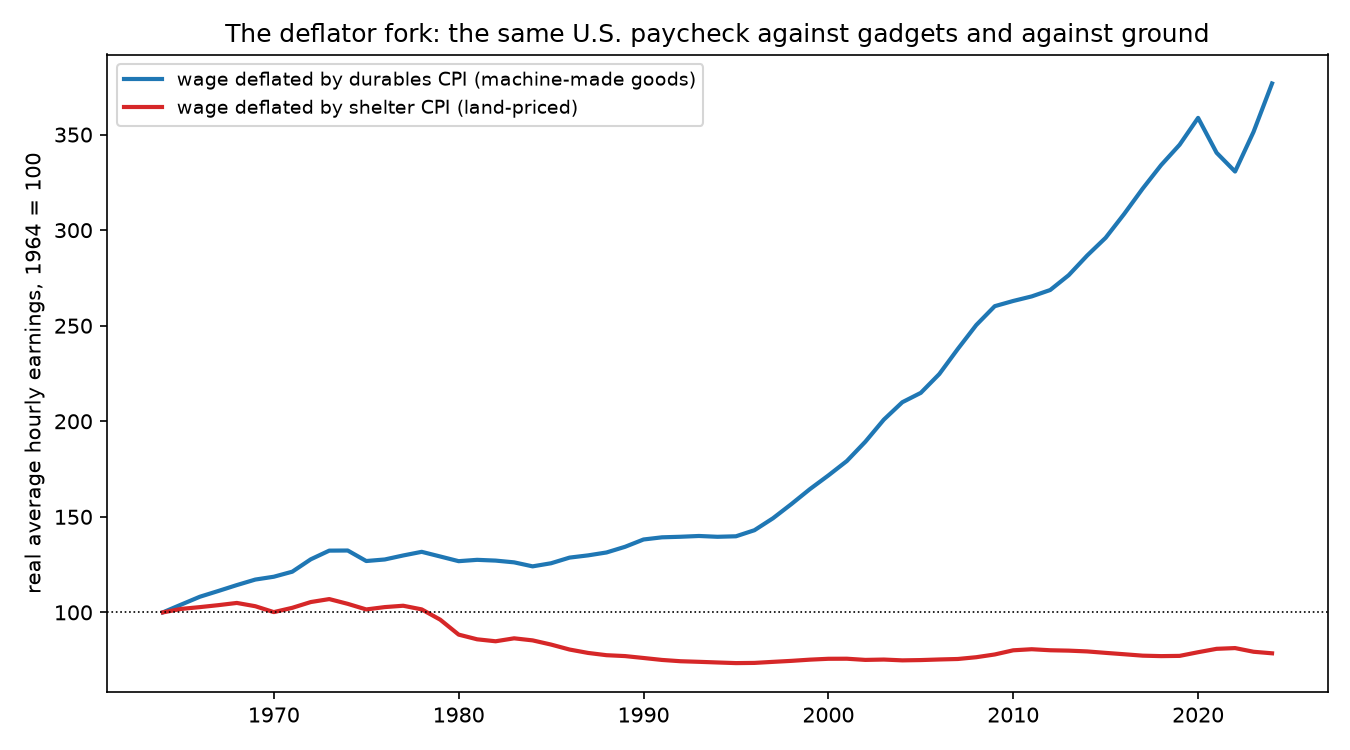
\includegraphics[width=0.88\linewidth]{figures/fig_deflator_fork.png}
\caption{The real-wage fork: U.S. average hourly earnings (production and nonsupervisory) deflated by the durables CPI and by the shelter CPI, 1964 = 100, complete calendar years through 2024. The fork ratio reaches $4.8\times$.}
\label{fig:fork}
\end{figure}

\textbf{The floor's coverage.} Appendix~\ref{app:coverage} defines $\kappa$ as the fraction of one subsistence bundle that a full tax on site rents could finance per person. Figure~\ref{fig:kappa} measures aggregate site-rent flow against population times a costed subsistence bundle. The 2025 estimate is $\kappa=0.33$ [0.18--0.59], up from roughly 0.05 in the 1950s. The measures are intended as lower-bound constructions, and the physical ceiling remains land per head; Appendix~\ref{app:coverage} states both restrictions.

\begin{figure}[t!]
\centering
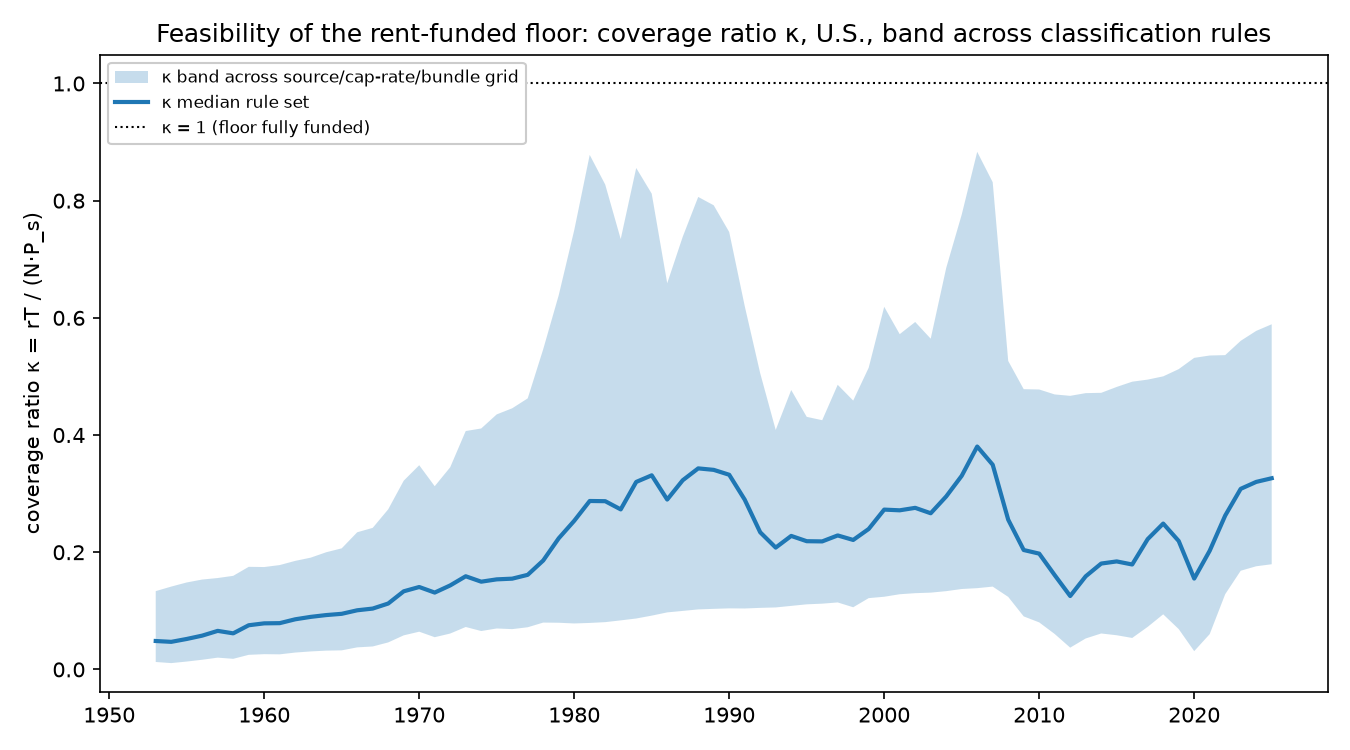
\includegraphics[width=0.88\linewidth]{figures/fig_kappa.png}
\caption{Coverage ratio $\kappa = rT/(N\cdot P_s)$ --- site rents $rT$ against population $N$ times the subsistence bundle's cost $P_s$ --- U.S., 1953--2025: median and min--max band across the land-source $\times$ capitalization-rate $\times$ bundle grid. Band width is substantially the capitalization-rate spread; the Z.1-residual members measure land as market value minus estimated structure replacement cost, an estimate known to be unreliable after 1995, and their business-structure coverage ends in 2020.}
\label{fig:kappa}
\end{figure}

\textbf{Financing versus production.} Consumption remains substantially more labor-financed than production is labor-intensive. In the common source-supported window, labor-origin resources finance 69.6\% of consumption in 2004 and 65.8\% in 2023, while full-chain human effort accounts for 48.9\% and 47.2\% of consumed production in the same years --- a gap of about nineteen percentage points at the end of the overlap (Figure~\ref{fig:labor-linkages}). The production account is the aggregate counterpart of the recursion: the human-effort share declines as machine-producing and machine-operating chains shed labor. Appendix~\ref{app:effort} gives the two accounts' definitions, sources, bounds, weaker long-run extensions, and mapping to the model.

\begin{figure}[t!]
\centering

\includegraphics[width=0.92\linewidth]{figures/fig_consumption_financing_and_human_effort.png}
\caption{Where labor enters U.S. consumption, 1950--2025. The upper series is the share of consumption spending financed from labor-origin resources; the lower is the share of consumed production that resolves into human effort through the full production chain. Markers identify the strongest source-supported windows: annual BEA income-source profiles for financing in 2004--2023 and the BEA full-chain production benchmark in 1997--2023. Outer years are weaker extensions. In the common source-supported window, consumption remains substantially more labor-financed than production is labor-intensive.}
\label{fig:labor-linkages}
\end{figure}

Two empirical tests remain open. Payroll-tax incidence can be normalized to a common pass-through definition and read, in this model, as repeated evidence on the inverse slope of the task schedule; the long welfare-ratio and land-share records can test the historical regime interpretation of Section~\ref{sec:history}. A principal rival for the shelter leg is zoning and other supply restriction. That changes the level of scarcity and is therefore central for policy, but it does not change the accounting mechanism: the discriminating evidence is whether the fork varies systematically with local regulation and local exposure.

\section{Possible stabilizers}\label{sec:stabilizers}

Three stabilizers can preserve wage purchasing power over scarce services, but they work through different margins. Human-essential tasks can persist by preference or by law; Appendix~\ref{app:human} shows that this can preserve aggregate labor income while leaving the median worker exposed. Institutions can reserve tasks for people outright, which is quantity rather than price protection. Supply expansion --- building, densifying, powering --- works on the other side of the model by loosening the terminal constraint and directly lowering $q$.

The wedge result behind that distinction is Acemoglu and Restrepo's (2026). Let a task pay a premium over the base wage --- a union premium, a licensing rent, an efficiency wage --- as a multiplicative wedge $\mu (x) > 1$. Labor then holds the task only while $w \le c\cdot \gamma (x)/\mu (x)$: allocation runs on the wedge-deflated schedule, a premium raises its own task's flip priority one-for-one, and automation is directed at the best-paid versions of each job --- their targeting result, with the documented losses concentrated in the 70th--95th within-group percentiles. A wage premium therefore increases the incentive to automate the protected task; protection survives only in quantity form --- a scope-of-practice rule extended to software, an enforceable automation ban, a mandated human in the loop. Under pressure, protection converts from price form toward legal form, and adoption at legally blocked tasks turns punctuated: nothing moves while the saving from flipping runs below the cost of confrontation; past it, everything the rule covers flips at once.

\section{Implications for artificial intelligence, and conclusion}\label{sec:ai}

AI is the first technology that very plausibly moves both automation margins at once. It lowers $\gamma (x^*)$ wherever models reach parity at final tasks --- and it lowers $\lambda$, because software generation, chip design, datacenter operation, logistics, and research are themselves the machine sector's labor. The strong scenario of this paper requires both empirically: capability closing faster than reinstatement replenishes it, and the machine-production network shedding its own labor. If neither happens, the flat limit is a curiosity. If both do, the model predicts that the marginal replacement value of labor falls while the outside option deteriorates in the scarce inputs required for exit, and that the gains from automation increasingly accrue as rents on sites, power, water, minerals, and legally protected scarce assets --- not on reproducible capital, whose price the recursion competes away. The prediction for the AI buildout itself is specific: model weights are ideas, copiable and distillable (distillation: cheaply training one model to imitate another); the durable balance-sheet items are the datacenters, the land under them, the power contracts, and the water rights.

One timing fact changes the policy conclusion: the same rise in $q$ that erodes the wage's purchasing power over scarce services and lowers the exit option also raises the value of the rent base. Coverage of a rent-funded floor has climbed from 0.05 to one-third in seventy years, while 0.68 of tax revenue remains wage-linked. Proposition~\ref{prop:welfare} resolves that mismatch in the limit with a fixed-base rent tax funding a transfer that leaves the compensated work--exit margin unchanged. Whether the economy approaches that limit is empirical; the transition is not costless or automatic. Appendix~\ref{app:fiscal} therefore asks which bases can finance the path and how the incidence changes before the limit is reached.

The effort account narrows the central empirical question. Consumed production is already substantially less labor-linked than the resources financing it, and the full-chain human-effort share is lower at the end of its source-supported window than at the beginning. That aggregate evidence does not yet isolate the machine-sector $\lambda$. The remaining question is therefore sharper: is the machine-production recursion itself becoming less wage-linked and more scarcity-linked, and is the same scarcity eroding the value of exit?

\appendix
\counterwithin{proposition}{section}
\titleformat{\section}{\normalfont\Large\bfseries}{Appendix~\thesection.}{0.6em}{}

\section{The environment and assignment equilibrium}\label{app:environment}

The economy below generalizes the model of Sections~\ref{sec:model}--\ref{sec:floor}; the main text is the case with every extension absent --- one machine type, no reserved tasks, no government --- and each appendix relaxes one restriction. Notation is defined here once, and the machine sector's general form --- many machine types, durability --- is stated here as well. Every result is proved in the configuration it states, with the remaining restrictions in place; existence for the unrestricted economy is not claimed.

\textbf{Tasks and technology.} A final good requires a continuum of tasks $x\in[0,1]$ in equal amounts (Section~\ref{sec:model}). One human-hour completes $\gamma _L(x)$ units of task $x$, one machine-hour $\gamma _M(x)$; relative human productivity is $\gamma (x) = \gamma _L(x)/\gamma _M(x)$. A set $H$ of measure $|H| \ge 0$ is closed to machines --- by capability, preference, or law (Appendix~\ref{app:human}).

\textbf{Machines.} Machine services are produced. With one machine type, a unit takes $a$ units of machine services, $\lambda$ labor-hours, and $b$ units of non-produced services renting at $r$ (Section~\ref{sec:model}). With many produced inputs, $\mathbf{c}$ is the vector of their prices, $\mathbf{A}$ the produced-input requirements matrix, $\boldsymbol{\Lambda}$ the labor requirements, $\mathbf{B}$ the requirements of terminal inputs with rent vector $\mathbf{r}$; free entry gives $\mathbf{c} = \mathbf{A}\mathbf{c} + \boldsymbol{\Lambda}w + \mathbf{B}\mathbf{r}$, hence $\mathbf{c} = (I-\mathbf{A})^{-1}(\boldsymbol{\Lambda}w + \mathbf{B}\mathbf{r})$ provided the spectral radius of $\mathbf{A}$ is below one --- the many-good statement of net reproduction. The scalar text carries the full logic: produced-input prices pass backward until anchored by factors outside the recursion and, during transition, by the labor still embodied in produced inputs. The task margin selects which machine type is the binding alternative at $x^*$: the one minimizing delivered task cost, and the threshold condition holds against that minimum. Free entry prices every produced input at unit cost.

\textbf{Durability, time preference, horizon.} With one-period building and time preference $\rho$ (the interest rate, distinct from the rent $r$), the $\lambda = 0$ recursion becomes $c = br(1+\rho )/(1 - a(1+\rho ))$, finite iff $a(1+\rho ) < 1$; with wear at rate $\delta$, the user-cost recursion gives $c = br(\rho +\delta )/(1 - a(\rho +\delta ))$. With $\lambda > 0$ the same closures hold with the recipe's labor priced at the margin: $c = br(1+\rho )/(1 - (1+\rho )(a + \lambda \gamma (x^*)))$ and $c = br(\rho +\delta )/(1 - (\rho +\delta )(a + \lambda \gamma (x^*)))$, finite iff $(1+\rho )(a + \lambda \gamma (x^*)) < 1$, respectively $(\rho +\delta )(a + \lambda \gamma (x^*)) < 1$. The added term is interest --- the wage of waiting --- competitive and real; it extends the income taxonomy without changing any destination. (These displays are computer-algebra-checked.) Whether an input is terminal is horizon-relative: transformer capacity is terminal over five years and produced over twenty; land is terminal at every horizon. The propositions hold per horizon with the classification made explicit, and our permanent-case claims use land alone.

\textbf{Non-produced inputs.} Terminal stocks are fixed: $T_j$ at rent $r_j$ where several matter (Section~\ref{sec:fiscal}), land the permanent case --- parcels of heterogeneous quality, reservation rent zero at the idle margin, rent schedule $r(z)$ over parcels $z$ (Appendix~\ref{app:landonly}). Land serves machine production and households: housing, and the $h_e$ units an independent exit requires.

\textbf{People.} $N$ workers each supply one hour or exit; types may differ in schedules and outside options (heterogeneous workers, below). Exit yields the keep $s_0$ on $h_e$ units of land, degrading to the dependency floor $\underline{s}$: $s(q) = \max(s_0 - q\cdot h_e, \underline{s})$ (Section~\ref{sec:floor}). Households spend on the machine-made good and direct land services, CES with weight $\alpha$ and elasticity $\sigma$; $\sigma = 1$ is Appendix~\ref{app:landonly}'s Cobb--Douglas, and general $\sigma$ is stated there.

\textbf{Government.} Four instruments: a payroll tax $\tau _w$ (Section~\ref{sec:fiscal}); a tax $\tau _R$ on pure ownership rents of terminal factors, returned as the uniform per-person transfer $d = \tau _R R/N$ (Section~\ref{sec:fiscal}); a uniform consumption tax (Appendix~\ref{app:mix}); and a transfer program --- the pair $(m_w,m_e)$, what it pays per period in work and out of it (Appendix~\ref{app:conditionality}).

\textbf{Equilibrium.} An equilibrium of a configuration is prices $(w,c,r(z))$, a task assignment, and a participation set such that every task is held by the input that costs less at ruling prices, free entry holds in machine production, the land market clears, and each worker participates exactly when work beats exit at the ruling prices and transfers. The configurations:

\begin{center}
{\small
\begin{tabular}{l p{8.6cm}}
\toprule
Where & Configuration \\
\midrule
Main text, Sections~\ref{sec:model}--\ref{sec:limit} & one machine type, $H = \emptyset$, no government \\
Section~\ref{sec:fiscal} & the rent tax and transfer $(\tau _R,d)$; the payroll contrast $\tau _w$ \\
Appendix~\ref{app:landonly} & the limit: $\gamma$ flat, $\lambda = 0, \rho = 0$; $\sigma = 1$, then general $\sigma$ \\
Appendix~\ref{app:fiscal} & government in full, sloped regime \\
Appendix~\ref{app:human} & $H$ of positive measure; $\gamma \to 0$ outside $H$ \\
\bottomrule
\end{tabular}
}
\end{center}

\begin{lemma}[existence and uniqueness]\label{lem:existence}
With the relabeled $\gamma$ continuous and strictly increasing where labor is employed, an equilibrium pair $(w, x^*)$ exists and is unique for any participant count; on a flat stretch the wage is pinned and only the assignment of identical-cost tasks is indeterminate, with nothing riding on it.
\end{lemma}

\begin{proof}
Absorbing more participants requires labor to hold more tasks, so the market-clearing wage $c\cdot \gamma (x^*(N_a))$, with $N_a$ the participant count, is continuous and strictly decreasing in $N_a$; participation supply is a step at $s$. A strictly decreasing continuous curve crosses a step exactly once, with Proposition~\ref{prop:margin}(iii) resolving the below-$s$ branch; flat stretches pin the wage at $c\cdot \bar{\gamma}$ and leave free only a measure-preserving relabeling.
\end{proof}

\textbf{The joint system.} With the recursion active, $c$ depends on $x^*$ through the machine sector's wage bill: $c(x^*) = br/(1 - a - \lambda \gamma (x^*))$ given $r$, and $w(x^*) = \gamma (x^*)\cdot c(x^*)$. Both are increasing in $\gamma (x^*)$ on the viable set $(\partial w/\partial \gamma (x^*) = br(1-a)/(1-a-\lambda \gamma (x^*))^2 > 0)$, so the market-clearing wage remains strictly decreasing in the participant count and Lemma~\ref{lem:existence}'s crossing argument survives unchanged. Full equilibrium adds land clearing and the endogenous outside option: $r$ clears the fixed land stock against machine-sector demand plus housing demand, and $s=s(q)$ follows Proposition~\ref{prop:exit}. At a given $r$, the monotonicity needed for the labor-market crossing remains intact. With $r$ endogenous, existence is established only in the scopes stated here: the exact flat-limit closure of Appendix~\ref{app:landonly} and a numerical worked configuration for the joint sloped system, in which the check files solve $(w,c,r,x^*)$ with land and labor clearing simultaneously. A general fixed-point proof for the joint sloped system is not claimed. Labor-market clearing counts both employments: final tasks plus $\lambda$ hours per unit of gross machine services.

\textbf{Heterogeneous workers.} With type-specific schedules and outside options, every proposition applies type by type; the aggregate schedule is the upper envelope of type schedules and the participation step becomes a distribution of steps. Floor statements refer to the bottom of the support.

\section{The land-only closure}\label{app:landonly}

Take Appendix~\ref{app:environment}'s economy to the flat, fully recursively automated case: $\gamma$ flat at $\bar{\gamma}$, $\lambda=0$, $\rho=0$, one terminal factor (land, homogeneous here; the heterogeneous case below), preferences at $\sigma = 1$ --- Cobb--Douglas with share $\alpha$ --- the stock $T$ jointly held and split between production use $T_P$ and housing $T_H$.

\begin{proposition}[closure and conservation of rents]\label{prop:landonly}
(i) Equilibrium exists with unique real allocation: $T_H = \alpha T, T_P = (1-\alpha )T$, final-good output $Y = (1-a)(1-\alpha )T/(b\bar{\gamma}\bar{L})$. (ii) The entire goods bill is production-land rent and national income is aggregate site rent identically: $pY = rT_P, pY + rT_H = rT$. (iii) Market clearing reproduces the cost-side relative price $r/p = (1-a)/(b\bar{\gamma}\bar{L})$: demand side and cost side agree on the same number.
\end{proposition}

\begin{proof}
Gross machine services solve $X = \bar{\gamma}\bar{L}Y + aX$, so $X = \bar{\gamma}\bar{L}Y/(1-a)$ and production land demand is $bX$. Substituting $p = br\bar{\gamma}\bar{L}/(1-a)$ gives $pY = r bX = rT_P$: goods spending passes through the zero-profit machine sector and accrues, all of it, to production land. Land being the only primary factor, household income is $rT$; Cobb--Douglas shares give $rT_H = \alpha rT$ and $pY = (1-\alpha )rT$; clearing pins $Y$ and dividing returns (iii).
\end{proof}

Dissipation is migration, by construction: the obvious escape --- automation's value dissipating into consumer surplus at collapsing prices --- is blocked, because prices do collapse \emph{and} the identity holds; what collapses is $p$ relative to $r$, never rent's claim on the flow of spending. \textbf{Heterogeneous parcels:} with a rent schedule over parcels in use and reservation rent zero at the idle margin, $rT$ reads $\int r(z)\,dz$ over parcels and nothing changes: the proposition requires only that spending, wherever it goes, crosses a site. \textbf{Labor still present in the flat regime:} the identity weakens to ``all non-wage income is site rent,'' GDP $= N\cdot c\bar{\gamma} + rT$, recovering the full identity as $\bar{\gamma} \to 0$. \textbf{Feedback:} a rent-funded floor is spent partly on land services, lifting $r$ and the base $rT$ --- favorable in direction, distribution-dependent in size; claimed as tendency only.

\textbf{General $\bm{\sigma}$.} With the general elasticity $\sigma$ of Appendix~\ref{app:environment}'s preferences between goods and land services, the land share of expenditure becomes
\begin{equation}\label{eq:ces-share}
\alpha (q) = \alpha q^{1-\sigma} / (\alpha q^{1-\sigma} + 1 - \alpha ),
\end{equation}
and as automation sends $q$ up (Proposition~\ref{prop:fork}(ii)): $\alpha (q) \to 1$ for $\sigma < 1$ --- complements; housing takes the whole budget and the fork binds --- while $\alpha (q) \to 0$ for $\sigma > 1$ and substitution defuses it. The climbing shelter share of low-income budgets is the $\sigma < 1$ signature.

\section{Fiscal transition in the sloped regime}\label{app:fiscal}

The main text gives the fiscal result in the flat limit. This appendix collects the transition results for a sloped task schedule: conditionality, payroll-tax incidence, rent-base coverage, and a reduced-form index of the residual distortionary financing need.

\subsection{Conditionality}\label{app:conditionality}

Let a transfer program pay $(m_w,m_e)$ in work and exit. The worker compares $w+m_w$ with $s+m_e$, so the compensated participation margin depends only on
\[
\Delta=m_w-m_e,
\qquad
w\ge s-\Delta.
\]
An in-work benefit $(\Delta>0)$ lowers the reservation wage and expands participation. In the sloped regime, part of the benefit is therefore offset by a lower equilibrium wage through the task margin. In the flat regime, an in-work subsidy can preserve hours whose replacement value lies below the outside option. An out-of-work benefit $(\Delta<0)$ raises the reservation wage and taxes the first hour of work; as the wage distribution compresses toward the floor, more workers enter any fixed withdrawal band. Within this two-payment class, $\Delta=0$ --- the same transfer in and out of work --- is the unique case with zero compensated participation effect. Income effects remain separate and are not set to zero by the identity.

\subsection{Funding and the incidence dial}\label{app:funding}

At the flat limit, a payroll-funded transfer is the closed loop of Section~\ref{sec:fiscal}. Away from the limit, let $\varepsilon_D$ and $\varepsilon_S$ denote labor-demand and participation elasticities in absolute value. Workers bear
\[
\frac{\varepsilon_D}{\varepsilon_D+\varepsilon_S}
\]
of a payroll tax, so the same fraction of a wage-funded transfer is circular: it is taken from the net wage and returned as the transfer. Proposition~\ref{prop:margin}(ii) maps $\varepsilon_D$ to the inverse slope of the task schedule at the margin. Payroll-incidence estimates can therefore be read, within the model, as evidence about flattening. By contrast, a tax on pure rents of a fixed factor cannot shrink that factor's supply; this production-efficiency property does not require the flat limit.

\subsection{Feasibility: the coverage ratio}\label{app:coverage}

Let one person's subsistence bundle contain $g_s$ units of goods and $h_s$ units of land services, so
\[
P_s=pg_s+rh_s.
\]
Full capture of site rent pays $rT/N$ per person. With $q=r/p$, the coverage ratio is
\[
\kappa=\frac{rT}{NP_s}
      =\frac{qT}{N(g_s+qh_s)}.
\]
It is strictly increasing in $q$ and converges to the physical ceiling $T/(Nh_s)$. Full coverage, $\kappa\ge1$, is possible at a finite relative price iff $T>Nh_s$, in which case
\[
q\ge q^*=\frac{Ng_s}{T-Nh_s}.
\]
The fiscal constraint is therefore a land constraint in disguise: the direct plus embodied land content of $N$ subsistence bundles must fit inside the available stock. Figure~\ref{fig:kappa} measures $\kappa$ at roughly 0.05 in the 1950s and 0.33 [0.18--0.59] in 2025.

For illustration, set $T=100$ and $g_s=h_s=1$. At $q=10/9$, fifty people are covered with room to spare $(\kappa=20/19)$; with eighty people, full coverage requires $q\ge4$; with 120 people, the physical ceiling is below one and full coverage is impossible at any $q$.

\subsection{The race with enclosure}\label{app:race}

Proposition~\ref{prop:exit}'s independent exit ends when rising rents exhaust the keep,
\[
q_{\mathrm{enc}}=\frac{s_0-\underline{s}}{h_e}.
\]
The rent-funded floor arrives at $q^*$. The natural floor therefore lasts until the fiscal replacement is available iff $q_{\mathrm{enc}}\ge q^*$, equivalently
\[
N\le \frac{q_{\mathrm{enc}}T}{g_s+q_{\mathrm{enc}}h_s}.
\]
Otherwise a transition gap opens: the commons has disappeared before site rents can fund the full floor. In the worked example above, $q_{\mathrm{enc}}=1.5$ implies a threshold of 60 people. The cancellation result for a uniform transfer survives on either side of this threshold; what changes is whether the rent base is large enough to finance the target floor.

\subsection{The financing mix on the way down}\label{app:mix}

Until $\kappa$ reaches one, site rents alone cannot finance a full floor. A rent tax reaches site rents whether saved or consumed, but not other bottleneck profits or royalties. A broad consumption tax reaches those other financing sources as they fund consumption, but its labor-origin slice is distortionary in the same direction as a wage tax.

For a descriptive transition index, let $\varphi_C$ be the labor-origin financing share of consumption and normalize the full floor to one. If the distortionary cost of the residual consumption-tax requirement is quadratic in the rate, filling the non-distortionary rent base first leaves an index proportional to
\[
D=\varphi_C(1-\kappa)^2.
\]
Using the 2025 weak-extension central values $\varphi_C=0.64$ and $\kappa=0.33$ gives $D=0.29$; at $(\varphi_C,\kappa)=(0.50,0.60)$ it would be 0.08. This is an index, not a structural welfare estimate. As $\kappa$ rises and labor-origin financing falls, the residual distortionary financing need shrinks; in the land-only limit, consumption ultimately resolves into rent income by Proposition~\ref{prop:landonly}, and the mix question disappears.

\begin{center}
{\small
\begin{tabular}{p{5.4cm} p{3.5cm} p{4.8cm}}
\toprule
Object & Value (year) & Note \\
\midrule
Labor-origin financing share of PCE, $\varphi_C$ & 0.64 [0.54--0.81] (2025, weak extension) & 0.66 [0.53--0.80] in the 2023 source-profile window; $\approx 0.74$ in 1965 weak extension \\
Wage-linked share of tax revenue, $\varphi_G$ & 0.68 (2025) & 0.64 in 1965; $\approx 0.70$ by the mid-1980s, flat since \\
Work- or means-conditioned share of benefits & $\ge 0.84$; $\approx 0.99$ by withdrawal rule (2024) & the only sizable unconditional cash transfer is Alaska's dividend \\
Coverage ratio $\kappa$ (Appendix~\ref{app:coverage}) & 0.33 [0.18--0.59] (2025) & $\approx 0.05$ in the 1950s; land measures are lower-bound constructions \\
Transition financing index $D=\varphi_C(1-\kappa)^2$ & 0.29 (2025, weak-extension central values) & descriptive index, not a structural welfare estimate \\
\bottomrule
\end{tabular}
}
\end{center}

\begin{figure}[t!]
\centering
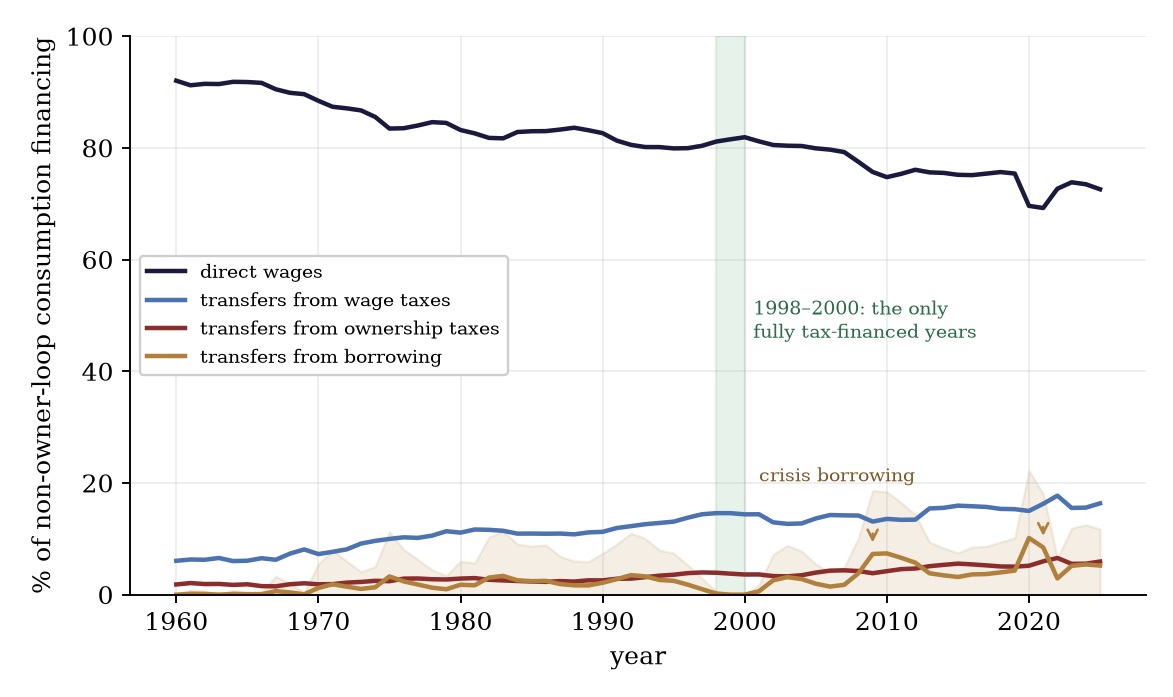
\includegraphics[width=0.88\linewidth]{figures/fig_fourway.png}
\caption{Financing of U.S. consumption outside the owner loop --- the slice financed directly by household capital income, owners consuming their own returns --- 1962--2025 (medians across the classification-rule grid; the shaded band spans deficit-attribution rules). Direct wages' share has fallen by about twenty percentage points in sixty years. Transfers grew on a funding mix that remained roughly one-quarter ownership-financed; the borrowed channel reached 19\% of transfers by 2025 and vanished only in 1998--2000. Funding attribution is pro-rata accounting, not estimated incidence.}
\label{fig:fourway}
\end{figure}

\section{Human-essential tasks}\label{app:human}

Let Appendix~\ref{app:environment}'s set $H$ have positive measure $|H|$: tasks machines cannot hold --- by capability residue, by verified preference for human hands, or by law --- with $H$-wage $w_H$. Let machines grow unboundedly better at every task outside $H$: $\gamma (x) \to 0$ there, the stricter limit of Section~\ref{sec:limit}'s corollary confined to the tasks machines can hold. The machine rental $c$ stays pinned by the recursion; what vanishes is the per-task cost of machine work, $c/\gamma _M(x) = c\cdot \gamma (x)/\gamma _L(x)$. Aghion, Jones, and Jones (2019) raise the strongest stabilizer this paper faces: Baumol concentration --- expenditure concentrating on the sector whose costs refuse to fall (Baumol 1967), here the human-essential set --- can preserve labor's share indefinitely. Proposition~\ref{prop:baumol} grants the mechanism its theorem and makes its premise explicit.

\begin{proposition}[Baumol concentration]\label{prop:baumol}
(i) Any good whose task list contains $H$ has unit cost tending to $|H|\cdot w_H/\gamma _L$ as $\gamma \to 0$ outside $H$: labor's share of its cost tends to one. (ii) Under CES substitution $\sigma _H$ between $H$-content and $H$-light substitutes, the expenditure share of $H$-content tends to 1 if $\sigma _H < 1$, to the taste weight if $\sigma _H = 1$, and to 0 if $\sigma _H > 1$. (iii) On the $\sigma _H < 1$ branch with three categories (machine-made goods, land services, $H$-labor), end-state expenditure splits between the two non-collapsing categories --- land services and $H$-labor --- and labor's aggregate share tends to the $H$-share of that split. Our baseline is exactly the $H = \emptyset$ edge of this result.
\end{proposition}

\begin{proof}
(i) $H$-tasks cost $|H|\cdot w_H/\gamma _L$ whatever machines do; each task outside $H$ costs $c\cdot \gamma (x)/\gamma _L(x)$, and the recursion keeps $c$ bounded as $\gamma$ falls (Proposition~\ref{prop:replacement}), so the remainder vanishes with $\gamma$. (ii) is Appendix~\ref{app:landonly}'s share display with $q$ read as the relative price of $H$-content: the costlier category's share rises with its relative price iff $\sigma _H < 1$, and by (i) that relative price diverges. (iii) A $H$-free good's price vanishes by (i) at $|H| = 0$, so for $\sigma _H < 1$ its share vanishes, leaving the displayed split; setting the $H$ taste weight to zero returns the baseline.
\end{proof}

Two anchors, and a hollowness result. \emph{Credence (the buyer cannot verify provenance):} preference-based membership binds only if provenance can be verified: suppose buyers carry a taste premium for verified human work, verification catches a false claim with probability $v$, and a caught claim pays a penalty $f$.

\begin{lemma}[the fraud bound]\label{lem:fraud}
A premium on verified human work is sustainable only up to $v\cdot f/(1-v)$: at any higher premium, false claiming is profitable in expectation and entry by fakes competes the premium away. The bound rises in $v$ and in $f$, diverges as $v \to 1$, and collapses to zero as $f \to 0$ for every $v < 1$.
\end{lemma}

\begin{proof}
A false claimant earns the premium with probability $1 - v$ and pays $f$ with probability $v$; expected profit is nonpositive iff the premium is at most $v\cdot f/(1-v)$. The comparative statics and limits are elementary.
\end{proof}

With price-only enforcement $(f \to 0)$ the bound collapses for every $v < 1$: certified-human markets unravel through fakes, not robots. $H$'s durable core is what law reserves plus what co-presence verifies --- being in the room, where faking is impossible rather than merely punished. \emph{Superstars:} within $H$, the broadcastable fraction $\psi$ of demand concentrates on top performers (Rosen 1981) while only the co-present remainder is rationed by human capacity.

\begin{lemma}[superstar concentration]\label{lem:superstar}
Let the broadcastable fraction $\psi$ of $H$-expenditure accrue to a set of performers of measure zero, and let the co-present remainder be shared uniformly across the $H$-workforce. The mean $H$-income is unchanged, and the median $H$-income is $(1-\psi )$ times the mean.
\end{lemma}

\begin{proof}
Total $H$-income equals $H$-expenditure whatever its division; the stars carry the fraction $\psi$ on measure zero, every other worker receives the uniform share $(1-\psi )$ times the mean, and a measure-zero top moves no quantile below the top.
\end{proof}

Wherever $H$ employs a minority the economy-wide median worker holds no $H$-task at all, and on the $\sigma _H < 1$ branch the aggregate labor share can persist, even approach one, while the median wage collapses to the floor: aggregate rescue, median collapse. The Baumol case also raises the floor's price: care and teaching put human hours in the subsistence bundle. Extend \ref{app:coverage}'s bundle with $n_s$ hours of $H$-service and coverage becomes $\kappa = qT/(N\cdot (g_s + n_s\cdot w_H/p + q\cdot h_s))$ --- below the $H$-free ratio at every $q$, and further below as the $H$-hour's price rises.

\section{The financing and production accounts}\label{app:effort}

Section~\ref{sec:measurement} quotes two shares; this appendix defines and constructs them. The \emph{labor-origin financing share} asks where the purchasing power used for personal consumption originates. The \emph{full-chain human-effort share} asks how much of the purchaser-price value of consumed production resolves into human labor after intermediates are traced recursively.

For 2004--2023 the financing account uses annual BEA source distributions ranked by equivalized disposable income. Spending beyond current disposable income is kept in an intertemporal bucket rather than assigned to current labor; within current-financed spending, tax incidence and allocation across fungible resources are partially identified and reported as bounds. The labor-origin financing share is 69.6\% [59.8--83.1] in 2004 and 65.8\% [52.7--80.1] in 2023; the weaker 2025 extension is 64.2\% [54.1--81.3].

The production account instead follows the purchaser-price dollar through the production chain. Its source-supported BEA benchmark covers 1997--2023: human effort is 50.1\% of consumed production in 1997 and 47.2\% in 2023. Outside that window, a five-specification product-composition model supplies only a weaker extension, at 66.4\% [61.3--68.6] in 1950 and 46.2\% [45.1--47.4] in 2025. Figure~\ref{fig:labor-linkages} marks the source-supported windows explicitly.

The common measured window is enough for the main point. In 2004, labor-origin resources finance 69.6\% of consumption while human effort accounts for 48.9\% of consumed production; in 2023 the shares are 65.8\% and 47.2\%. The gap is about nineteen percentage points at the end of the overlap. The long extension suggests that the separation is newer than the postwar starting point, but that inference inherits the weaker status of the outer series.

\textbf{Mapping back to the model.} The production account corresponds to the broader recursion $\mathbf{c}=\mathbf{A}\mathbf{c}+\boldsymbol{\Lambda}w+\mathbf{B}\mathbf{r}$ of Appendix~\ref{app:environment}, not to the scalar $\lambda$ in the one-sector machine recipe. Recursive automation predicts a declining human-effort component as machine-producing and machine-operating chains shed labor; the aggregate series is evidence about that direction. The financing account supplies the transition share $\varphi_C$ used in Appendix~\ref{app:mix}: 0.658 [0.527--0.801] in the last source-profile year, 2023, and 0.642 [0.541--0.813] in the weaker 2025 extension. Separately, 0.68 of tax revenue is wage-linked in 2025.

\section*{References}

{\small\singlespacing
\refentry{Acemoglu, D., and D. Autor (2011). ``Skills, Tasks and Technologies: Implications for Employment and Earnings.'' In \emph{Handbook of Labor Economics}, vol. 4B. Elsevier.}
\refentry{Acemoglu, D., and P. Restrepo (2018). ``The Race between Man and Machine: Implications of Technology for Growth, Factor Shares, and Employment.'' \emph{American Economic Review} 108(6): 1488--1542.}
\refentry{Acemoglu, D., and P. Restrepo (2022). ``Tasks, Automation, and the Rise in U.S. Wage Inequality.'' \emph{Econometrica} 90(5).}
\refentry{Acemoglu, D., and P. Restrepo (2026). ``Automation and Rent Dissipation: Implications for Wages, Inequality, and Productivity.'' \emph{The Quarterly Journal of Economics} 141(2): 1521--1579.}
\refentry{Aghion, P., B. F. Jones, and C. I. Jones (2019). ``Artificial Intelligence and Economic Growth.'' In A. Agrawal, J. Gans, and A. Goldfarb (eds.), \emph{The Economics of Artificial Intelligence}, University of Chicago Press.}
\refentry{Allen, R. C. (2001). ``The Great Divergence in European Wages and Prices from the Middle Ages to the First World War.'' \emph{Explorations in Economic History} 38(4): 411--447.}
\refentry{Arnott, R. J., and J. E. Stiglitz (1979). ``Aggregate Land Rents, Expenditure on Public Goods, and Optimal City Size.'' \emph{The Quarterly Journal of Economics} 93(4): 471--500.}
\refentry{Arrow, K. J. (1951). ``An Extension of the Basic Theorems of Classical Welfare Economics.'' In \emph{Proceedings of the Second Berkeley Symposium on Mathematical Statistics and Probability}, University of California Press.}
\refentry{Autor, D. (2015). ``Why Are There Still So Many Jobs? The History and Future of Workplace Automation.'' \emph{Journal of Economic Perspectives} 29(3).}
\refentry{Autor, D., and D. Dorn (2013). ``The Growth of Low-Skill Service Jobs and the Polarization of the US Labor Market.'' \emph{American Economic Review} 103(5): 1553--1597.}
\refentry{Autor, D., F. Levy, and R. J. Murnane (2003). ``The Skill Content of Recent Technological Change: An Empirical Exploration.'' \emph{The Quarterly Journal of Economics} 118(4): 1279--1333.}
\refentry{Baumol, W. J. (1967). ``Macroeconomics of Unbalanced Growth: The Anatomy of Urban Crisis.'' \emph{American Economic Review} 57(3): 415--426.}
\refentry{Bouscasse, P., E. Nakamura, and J. Steinsson (2025). ``When Did Growth Begin? New Estimates of Productivity Growth in England from 1250 to 1870.'' \emph{The Quarterly Journal of Economics} 140(2): 835--888.}
\refentry{Card, D., A. R. Cardoso, J. Heining, and P. Kline (2018). ``Firms and Labor Market Inequality: Evidence and Some Theory.'' \emph{Journal of Labor Economics} 36(S1).}
\refentry{Caselli, F., and A. Manning (2019). ``Robot Arithmetic: New Technology and Wages.'' \emph{American Economic Review: Insights} 1(1).}
\refentry{Clark, G. (2005). ``The Condition of the Working Class in England, 1209--2004.'' \emph{Journal of Political Economy} 113(6): 1307--1340.}
\refentry{Crafts, N. (2022). ``Slow Real Wage Growth during the Industrial Revolution: Productivity Paradox or Pro-Rich Growth?'' \emph{Oxford Economic Papers} 74(1): 1--13.}
\refentry{Diamond, P. A. (1982). ``Aggregate Demand Management in Search Equilibrium.'' \emph{Journal of Political Economy} 90(5).}
\refentry{Diamond, P., and J. Mirrlees (1971). ``Optimal Taxation and Public Production I: Production Efficiency.'' \emph{American Economic Review} 61(1).}
\refentry{George, H. (1879). \emph{Progress and Poverty.}}
\refentry{Grossman, G. M., and E. Rossi-Hansberg (2008). ``Trading Tasks: A Simple Theory of Offshoring.'' \emph{American Economic Review} 98(5).}
\refentry{Gruber, J. (1997). ``The Incidence of Payroll Taxation: Evidence from Chile.'' \emph{Journal of Labor Economics} 15(3, Part 2): S72--S101.}
\refentry{Hagedorn, M., and I. Manovskii (2008). ``The Cyclical Behavior of Equilibrium Unemployment and Vacancies Revisited.'' \emph{American Economic Review} 98(4): 1692--1706.}
\refentry{Hall, R. E. (2005). ``Employment Fluctuations with Equilibrium Wage Stickiness.'' \emph{American Economic Review} 95(1).}
\refentry{Hémous, D., and M. Olsen (2022). ``The Rise of the Machines: Automation, Horizontal Innovation, and Income Inequality.'' \emph{American Economic Journal: Macroeconomics} 14(1).}
\refentry{Hoynes, H., and J. Rothstein (2019). ``Universal Basic Income in the United States and Advanced Countries.'' \emph{Annual Review of Economics} 11.}
\refentry{Jones, D., and I. Marinescu (2022). ``The Labor Market Impacts of Universal and Permanent Cash Transfers: Evidence from the Alaska Permanent Fund.'' \emph{American Economic Journal: Economic Policy} 14(2): 315--340.}
\refentry{Karabarbounis, L., and B. Neiman (2014). ``The Global Decline of the Labor Share.'' \emph{The Quarterly Journal of Economics} 129(1).}
\refentry{Knoll, K., M. Schularick, and T. Steger (2017). ``No Price Like Home: Global House Prices, 1870--2012.'' \emph{American Economic Review} 107(2).}
\refentry{Korinek, A., and J. E. Stiglitz (2019). ``Artificial Intelligence and Its Implications for Income Distribution and Unemployment.'' In A. Agrawal, J. Gans, and A. Goldfarb (eds.), \emph{The Economics of Artificial Intelligence}, University of Chicago Press.}
\refentry{Korinek, A., and D. Suh (2024). ``Scenarios for the Transition to AGI.'' NBER Working Paper 32255.}
\refentry{Kugler, A., and M. Kugler (2009). ``Labor Market Effects of Payroll Taxes in Developing Countries: Evidence from Colombia.'' \emph{Economic Development and Cultural Change} 57(2): 335--358.}
\refentry{Leontief, W. W. (1936). ``Quantitative Input and Output Relations in the Economic Systems of the United States.'' \emph{The Review of Economics and Statistics} 18(3): 105--125.}
\refentry{Lewis, W. A. (1954). ``Economic Development with Unlimited Supplies of Labour.'' \emph{The Manchester School} 22(2): 139--191.}
\refentry{Ljungqvist, L., and T. J. Sargent (2017). ``The Fundamental Surplus.'' \emph{American Economic Review} 107(9): 2630--2665.}
\refentry{Malthus, T. R. (1798). \emph{An Essay on the Principle of Population.}}
\refentry{Manning, A. (2003). \emph{Monopsony in Motion: Imperfect Competition in Labor Markets.} Princeton University Press.}
\refentry{Mas, A., and A. Pallais (2019). ``Labor Supply and the Value of Non-Work Time: Experimental Estimates from the Field.'' \emph{American Economic Review: Insights} 1(1): 111--126.}
\refentry{Moll, B., L. Rachel, and P. Restrepo (2022). ``Uneven Growth: Automation's Impact on Income and Wealth Inequality.'' \emph{Econometrica} 90(6).}
\refentry{Mortensen, D. T., and C. A. Pissarides (1994). ``Job Creation and Job Destruction in the Theory of Unemployment.'' \emph{The Review of Economic Studies} 61(3): 397--415.}
\refentry{Piketty, T., and G. Zucman (2014). ``Capital is Back: Wealth-Income Ratios in Rich Countries 1700--2010.'' \emph{The Quarterly Journal of Economics} 129(3).}
\refentry{Pissarides, C. A. (2000). \emph{Equilibrium Unemployment Theory.} 2nd ed., MIT Press.}
\refentry{Polanyi, K. (1944). \emph{The Great Transformation.}}
\refentry{Ricardo, D. (1817). \emph{On the Principles of Political Economy and Taxation.} Third edition, 1821, adds the chapter ``On Machinery.''}
\refentry{Rognlie, M. (2015). ``Deciphering the Fall and Rise in the Net Capital Share.'' \emph{Brookings Papers on Economic Activity.}}
\refentry{Romer, P. M. (1990). ``Endogenous Technological Change.'' \emph{Journal of Political Economy} 98(5): S71--S102.}
\refentry{Rosen, S. (1981). ``The Economics of Superstars.'' \emph{American Economic Review} 71(5).}
\refentry{Sachs, J. D., and L. J. Kotlikoff (2012). ``Smart Machines and Long-Term Misery.'' NBER Working Paper 18629.}
\refentry{Saez, E., B. Schoefer, and D. Seim (2019). ``Payroll Taxes, Firm Behavior, and Rent Sharing: Evidence from a Young Workers' Tax Cut in Sweden.'' \emph{American Economic Review} 109(5): 1717--1763.}
\refentry{Samuelson, P. A. (1966). ``A Summing Up.'' \emph{The Quarterly Journal of Economics} 80(4).}
\refentry{Shapiro, C., and J. E. Stiglitz (1984). ``Equilibrium Unemployment as a Worker Discipline Device.'' \emph{American Economic Review} 74(3): 433--444.}
\refentry{Shimer, R. (2005). ``The Cyclical Behavior of Equilibrium Unemployment and Vacancies.'' \emph{American Economic Review} 95(1): 25--49.}
\refentry{Sraffa, P. (1960). \emph{Production of Commodities by Means of Commodities.} Cambridge University Press.}
\refentry{Susskind, D. (2017). ``A Model of Technological Unemployment.'' Oxford Department of Economics Discussion Paper 819.}
\refentry{Uzawa, H. (1961). ``Neutral Inventions and the Stability of Growth Equilibrium.'' \emph{The Review of Economic Studies} 28(2): 117--124.}
\refentry{Zeira, J. (1998). ``Workers, Machines, and Economic Growth.'' \emph{The Quarterly Journal of Economics} 113(4).}
}

\bigskip\par\noindent\rule{0.35\linewidth}{0.4pt}\par\smallskip
\noindent{\footnotesize\singlespacing \textbf{Data and computation.} All U.S. figures are gross annual flows computed from BEA national accounts (annual NIPA series retrieved via FRED, 2026 vintage), with Federal Reserve Z.1 balance-sheet lines, BEA fixed-assets stocks, and the CPI for the coverage ratio, and HUD FY2025 fair-market rents for the ceiling grid. Series windows follow their sources: financing splits 1962--2025, coverage ratio 1953--2025, deflator fork 1964--2024 on complete calendar years, with the food comparison from the CPI food index (FRED CPIUFDNS) over the same window. Every arguable classification was computed under all defensible variants; reported values are medians with min--max bands across the rule grid. Flows are gross. The effort-accounting additions keep the financing side separate from production content. The financing series uses annual BEA source profiles ranked by equivalized disposable income in 2004--2023 with partial-identification bounds and weaker outer extensions. The production series uses the BEA WP2026-01 full-chain benchmark in 1997--2023 and a five-specification NIPA product-composition extension outside that window. Figure~\ref{fig:labor-linkages} marks the source-supported windows explicitly so the long-run extensions are not read as equivalent observations. \textbf{Notation.} The machine-recipe labor coefficient $\lambda$ is unrelated to the wage-linkage shares $\varphi _C, \varphi _G$ of Appendix~\ref{app:fiscal} and to Acemoglu--Restrepo's task-substitution elasticity $\lambda$; rent is $r$ (aggregate $R$) while the interest rate is $\rho$; the wedge $\mu$ appears only in Section~\ref{sec:stabilizers}; the CES elasticities are $\sigma$ (goods versus land services, Appendix~\ref{app:landonly}) and $\sigma_H$ ($H$-content versus substitutes, Appendix~\ref{app:human}); the human-essential set $H$ is unrelated to the housing subscript of $T_H$; and the outside option is denoted $s$; the common search-theory symbol $b$ is reserved here for the terminal-input coefficient, and the subscripts $\lo, \hi$ mark Section~\ref{sec:limit}'s low- and high-land-intensity consumption composites.\par}

\bigskip\par\noindent\rule{0.35\linewidth}{0.4pt}\par\smallskip
\noindent{\footnotesize\singlespacing \textbf{Verification.} Every proposition's algebra is checked by computer algebra (sympy) and its equilibrium claims against numerical instantiations; the check files ship with the repository. The full-automation chain --- the $\lambda = 0$ recursion, the closure identity, the fork, the funding and conditionality results, and the welfare pair --- is also stated and proved in Lean 4 (with the mathlib library), as are the $\lambda > 0$ closure and its comparative statics (Propositions~\ref{prop:replacement} and \ref{prop:fork}(i)--(ii)), the user-cost closures, Lemmas \ref{lem:fraud} and \ref{lem:superstar}, and Appendix~\ref{app:landonly}'s CES share limits. The composite pricing display and Proposition~\ref{prop:fork}(iv) are computer-algebra-checked and sit outside the Lean development. The Lean development carries an assumption manifest --- the enumerated hypotheses each proposition consumes --- and its statements are a translation of the paper's: the proofs are machine-checked, the translation is not. The joint-system fixed point of Appendix~\ref{app:environment} is outside the formalization, as stated there.\par}

\bigskip\par\noindent\rule{0.35\linewidth}{0.4pt}\par\smallskip
\noindent{\footnotesize\singlespacing \textbf{AI use.} This paper was written in collaboration with Claude (Anthropic). The theory and its central claims are the authors'; the formalization, proofs, computations, figures, and nearly all of the prose were drafted by Claude under the authors' direction and review. All data were pulled live from public sources; the code and data are public. Errors remain the authors'.\par}

\end{document}
